% **** Szablon pracy magisterskiej, licencjackiej lub inżynierskiej ****

\documentclass[polish,12pt,twoside,a4paper]{report}

% *************** Definicje stylu dokumentu ***************

% *********************************************************************************
% W pliku tym zdefiniowany jest wygl¹d dokumentu.
% Zmiany tutaj nie s¹ konieczne o ile nie zamierzasz zmieniaæ wygl¹du dokumentu.
% *********************************************************************************

% *************** Za³adowanie pakietów ***************
\usepackage[a4paper,twoside,left=2.0cm,right=1.5cm,top=1.5cm,bottom=1.5cm]{geometry}
\usepackage[T1]{fontenc}
%\usepackage[cp1250]{inputenc}
\usepackage[utf8]{inputenc}
\usepackage[polish]{babel}
\usepackage{amsmath}
\usepackage{amsfonts}
\usepackage{graphicx}
\usepackage{graphics}
\usepackage{times}
\usepackage{indentfirst}%wciecia a nowych akapitach

\selectlanguage{polish}

%szerokoœœ wciêæ
\setlength{\parindent}{1.25cm}

%numeracja stron
\usepackage{fancyhdr}
\pagestyle{fancy}
\fancyhf{} % usun biezace ustawienia pagin
\fancyhead[LE,RO]{ }
\fancyhead[LO]{ }
\fancyhead[RE]{ }
\fancyfoot[LE,RO]{\small\thepage}
\fancyfoot[LO]{ }
\fancyfoot[RE]{ }
\renewcommand{\headrulewidth}{0.0pt}
\renewcommand{\footrulewidth}{0.0pt}
\addtolength{\headheight}{0.0pt} % pionowy odstep na kreske
\fancypagestyle{plain}{%
\fancyhead{} % usun p. górne na stronach pozbawionych
% numeracji (plain)
\renewcommand{\headrulewidth}{0.0pt} % pozioma kreska
}

% *************** Definicje niektórych kolorów ***************
\usepackage{color}

\definecolor{greenyellow}   {cmyk}{0.15, 0   , 0.69, 0   }
\definecolor{yellow}        {cmyk}{0   , 0   , 1   , 0   }
\definecolor{goldenrod}     {cmyk}{0   , 0.10, 0.84, 0   }
\definecolor{dandelion}     {cmyk}{0   , 0.29, 0.84, 0   }
\definecolor{apricot}       {cmyk}{0   , 0.32, 0.52, 0   }
\definecolor{peach}         {cmyk}{0   , 0.50, 0.70, 0   }
\definecolor{melon}         {cmyk}{0   , 0.46, 0.50, 0   }
\definecolor{yelloworange}  {cmyk}{0   , 0.42, 1   , 0   }
\definecolor{orange}        {cmyk}{0   , 0.61, 0.87, 0   }
\definecolor{burntorange}   {cmyk}{0   , 0.51, 1   , 0   }
\definecolor{bittersweet}   {cmyk}{0   , 0.75, 1   , 0.24}
\definecolor{redorange}     {cmyk}{0   , 0.77, 0.87, 0   }
\definecolor{mahogany}      {cmyk}{0   , 0.85, 0.87, 0.35}
\definecolor{maroon}        {cmyk}{0   , 0.87, 0.68, 0.32}
\definecolor{brickred}      {cmyk}{0   , 0.89, 0.94, 0.28}
\definecolor{red}           {cmyk}{0   , 1   , 1   , 0   }
\definecolor{orangered}     {cmyk}{0   , 1   , 0.50, 0   }
\definecolor{rubinered}     {cmyk}{0   , 1   , 0.13, 0   }
\definecolor{wildstrawberry}{cmyk}{0   , 0.96, 0.39, 0   }
\definecolor{salmon}        {cmyk}{0   , 0.53, 0.38, 0   }
\definecolor{carnationpink} {cmyk}{0   , 0.63, 0   , 0   }
\definecolor{magenta}       {cmyk}{0   , 1   , 0   , 0   }
\definecolor{violetred}     {cmyk}{0   , 0.81, 0   , 0   }
\definecolor{rhodamine}     {cmyk}{0   , 0.82, 0   , 0   }
\definecolor{mulberry}      {cmyk}{0.34, 0.90, 0   , 0.02}
\definecolor{redviolet}     {cmyk}{0.07, 0.90, 0   , 0.34}
\definecolor{fuchsia}       {cmyk}{0.47, 0.91, 0   , 0.08}
\definecolor{lavender}      {cmyk}{0   , 0.48, 0   , 0   }
\definecolor{thistle}       {cmyk}{0.12, 0.59, 0   , 0   }
\definecolor{orchid}        {cmyk}{0.32, 0.64, 0   , 0   }
\definecolor{darkorchid}    {cmyk}{0.40, 0.80, 0.20, 0   }
\definecolor{purple}        {cmyk}{0.45, 0.86, 0   , 0   }
\definecolor{plum}          {cmyk}{0.50, 1   , 0   , 0   }
\definecolor{violet}        {cmyk}{0.79, 0.88, 0   , 0   }
\definecolor{royalpurple}   {cmyk}{0.75, 0.90, 0   , 0   }
\definecolor{blueviolet}    {cmyk}{0.86, 0.91, 0   , 0.04}
\definecolor{periwinkle}    {cmyk}{0.57, 0.55, 0   , 0   }
\definecolor{cadetblue}     {cmyk}{0.62, 0.57, 0.23, 0   }
\definecolor{cornflowerblue}{cmyk}{0.65, 0.13, 0   , 0   }
\definecolor{midnightblue}  {cmyk}{0.98, 0.13, 0   , 0.43}
\definecolor{navyblue}      {cmyk}{0.94, 0.54, 0   , 0   }
\definecolor{royalblue}     {cmyk}{1   , 0.50, 0   , 0   }
\definecolor{blue}          {cmyk}{1   , 1   , 0   , 0   }
\definecolor{cerulean}      {cmyk}{0.94, 0.11, 0   , 0   }
\definecolor{cyan}          {cmyk}{1   , 0   , 0   , 0   }
\definecolor{processblue}   {cmyk}{0.96, 0   , 0   , 0   }
\definecolor{skyblue}       {cmyk}{0.62, 0   , 0.12, 0   }
\definecolor{turquoise}     {cmyk}{0.85, 0   , 0.20, 0   }
\definecolor{tealblue}      {cmyk}{0.86, 0   , 0.34, 0.02}
\definecolor{aquamarine}    {cmyk}{0.82, 0   , 0.30, 0   }
\definecolor{bluegreen}     {cmyk}{0.85, 0   , 0.33, 0   }
\definecolor{emerald}       {cmyk}{1   , 0   , 0.50, 0   }
\definecolor{junglegreen}   {cmyk}{0.99, 0   , 0.52, 0   }
\definecolor{seagreen}      {cmyk}{0.69, 0   , 0.50, 0   }
\definecolor{green}         {cmyk}{1   , 0   , 1   , 0   }
\definecolor{forestgreen}   {cmyk}{0.91, 0   , 0.88, 0.12}
\definecolor{pinegreen}     {cmyk}{0.92, 0   , 0.59, 0.25}
\definecolor{limegreen}     {cmyk}{0.50, 0   , 1   , 0   }
\definecolor{yellowgreen}   {cmyk}{0.44, 0   , 0.74, 0   }
\definecolor{springgreen}   {cmyk}{0.26, 0   , 0.76, 0   }
\definecolor{olivegreen}    {cmyk}{0.64, 0   , 0.95, 0.40}
\definecolor{rawsienna}     {cmyk}{0   , 0.72, 1   , 0.45}
\definecolor{sepia}         {cmyk}{0   , 0.83, 1   , 0.70}
\definecolor{brown}         {cmyk}{0   , 0.81, 1   , 0.60}
\definecolor{tan}           {cmyk}{0.14, 0.42, 0.56, 0   }
\definecolor{gray}          {cmyk}{0   , 0   , 0   , 0.50}
\definecolor{black}         {cmyk}{0   , 0   , 0   , 1   }
\definecolor{white}         {cmyk}{0   , 0   , 0   , 0   } 

% *************** Koniec definicji stylu dokumentu ***************


%definicja przydatnych poleceń
\newcommand{\wydzial}{KOLEGIUM INFORMATYKI STOSOWANEJ}
\newcommand{\kierunek}{Kierunek: INFORMATYKA}
\newcommand{\specjalnosc}{Specjalność: PROGRAMOWANIE}
\newcommand{\autor}{Artem Usenko, Oleksandr Knyzhnyk}
\newcommand{\album}{Nr albumu studentów w68183, w61852}
\newcommand{\temat}{E-Szpital}
\newcommand{\promotor}{dr inż. Ewa Żesławska}
\newcommand{\typpracy}{PROJEKT Z PRZEDMIOTU "PROGRAMOWANIE OBIEKTOWE"}
\newcommand{\miasto}{Rzeszów}
\newcommand{\rok}{2024}

\begin{document}

% *************** Włączenie definicji pierwszych stron ***************
% *************** Strony tytułowe ***************

% ************************************************************
% W tym miejscu znajduje sie definicja wyglądu pierwszych stron:
% strony tytułowej, strony z oświadczeniem o treści pracy
% i strony ze spisem treści
% ************************************************************
% *************** Strona tytułowa ***************
%umieszczenie logo i nazwy uczelni

\parbox{65mm}{
\includegraphics[width=13.0cm, height=3.0cm]{logoWSIiZ}}

\vspace{10mm}
\begin{center}
{\Large{}\textbf{\wydzial}}
\end{center}
\vspace{10mm}
\noindent
\hspace{30mm}{\Large{}\textbf{\kierunek}}\\

\noindent
\hspace{30mm}{\Large{}\textbf{\specjalnosc}}
\vspace{30mm}
\begin{center}
	{\large{}\autor}\\
	{\large{}\album}\\
	\vspace{15pt}
	{\huge{}\textbf{\textit{\temat}}}\\
	\vspace{20pt}
	{\normalsize{}Promotor: \promotor}\\
	\vspace{100pt}
	{\LARGE{}\textbf{\typpracy}}\\
	\vspace{190pt}
	{\large{}\textbf{\miasto {} \rok}}
\end{center}



% *************** Część główna pracy ***************
\chapter*{Wstęp}

Medycyna w Polsce jest dobrze rozwinięta, ale nie zawsze osoby, potrzebujące pomocy, otrzymują tę pomoc w najszybszym czasie. W rankingu tak zwanego zrównoważonego rozwoju systemów ochrony zdrowia Polska zajmuje 25 miejsce na 28 państw UE. Wychodząc z tego, pomysł projektu polega na zwracaniu dodatkowej uwagi tematu zdrowia, który został na takim poziomie w 2020 roku, na którym był w 2012.

\begin{figure}[!ht]
	\centering
		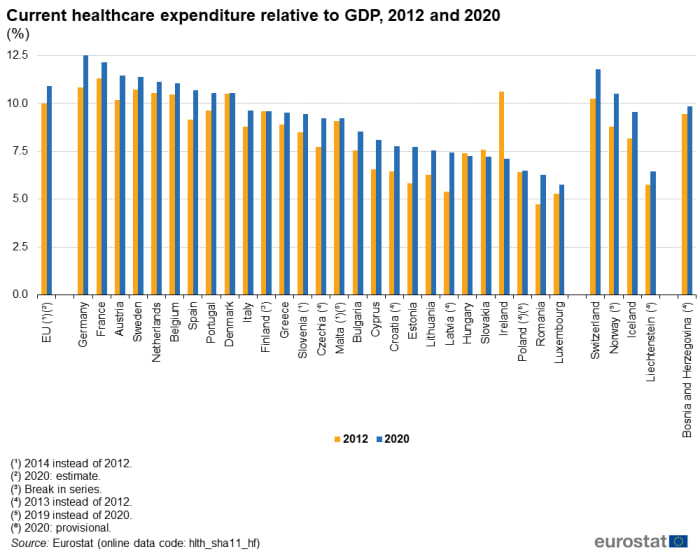
\includegraphics[width=16cm]{polska_med.jpg}
	\caption{\footnotesize Porównanie poziomu ochrony zdrowia pomiędzy krajami UE. Żródło: \cite{www-1}}
	\label{fig:plotend}
\end{figure}

Ignorowanie rozwoju tematów, powiązanych ze zdrowiem, może spowodować stracone życia, które udałoby uratować, gorsze wydarzenie o Polsce, jako o kraju w całości, powolnienie wykonywania prac we wszystkich obszarach biznesu i nie tylko.

\addcontentsline{toc}{chapter}{Wstęp}
\newpage
% ********** Rozdział 1 **********
\chapter{Wymagania projektu}
\section{Wymagania funkcjonalne i niefunkcjonalne}
\subsection{Wymagania funkcjonalne}

Z założeń projektu można powiedzieć, że funkcjonalne wymagania są:
\begin{itemize}
   \item Założenie konta
   \item Łatwe zarządzanie obszarzem bazy danych 
\item Sprawdzanie aptek w pobliżu
\item Sprawdzanie informacje o lekach
\item Wyświetlanie informacji o lekarzach
\item Recepty na leki 
\item Zważanie na przeciwwskazania
\item Głównie - wygodna, intuicyjnie zrozumiała nawigacja w aplikacji
\end{itemize}

W dodatek do tej listy można dodać bardziej szczegółowy opis. Założenie konta będzie potrzebować wprowadzanie i zapisywanie nowych danych do bazy danych.\newline Korzystanie z bazy danych do wyświetlenia nazwy, adresu i dt. informacje o wszystkich aptekach miasta; \newline Wyświetlanie danych o lekach, jako nazwa, producent, cena, dostępność, dawka, przeciwwskazania z uwagi na alergie. \newline Lekarze - imie, nazwisko, specjalność.
\subsection{Wymagania niefunkcjonalne}\label{przypisy}. 

Najbardziej wymagania niefunkcjonalne będą polegać na umówieniach z pracownikami i kierownictwem aptek, szpitalów i przychodzień. Jedną z najważniejszych możliwości, które musi udostępnić projekt "E-Szpital", jest łatwa komunikacja informacyjna w bazie danych, powiązana z każdym budynkiem, prowadzającym pomoc medyczną. \newline



% ********** Koniec rozdziału **********

\newpage
% ********** Rozdział 2 **********
\chapter{Tytuł rozdziału}


\section{Struktura projektu}
\begin{figure}[!ht]
	\centering
		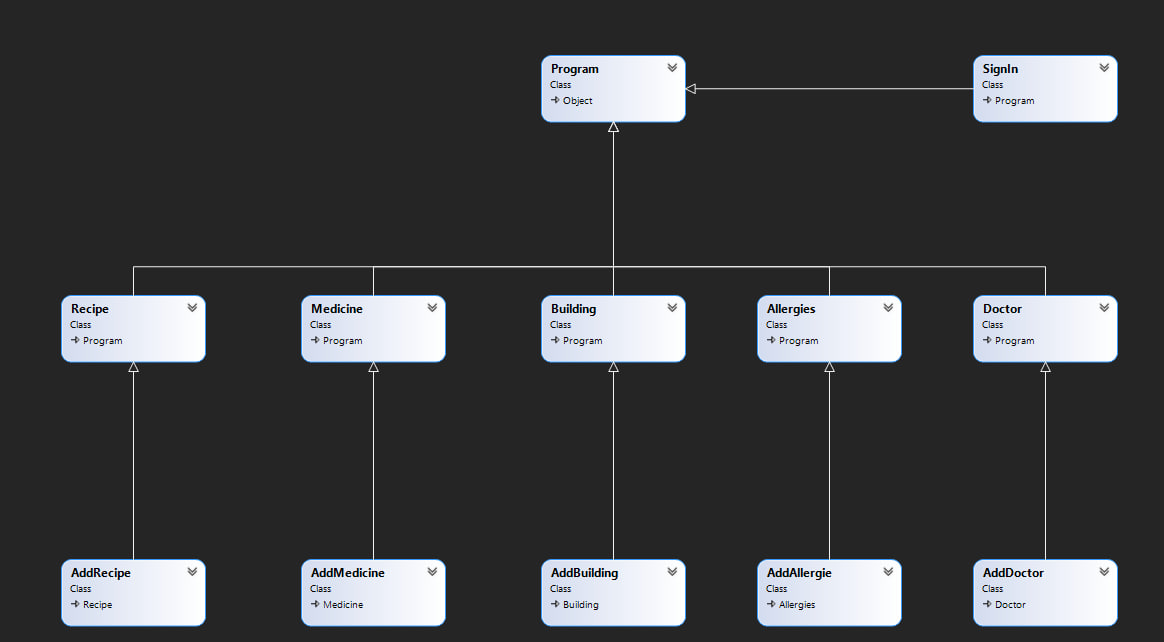
\includegraphics[width=16cm]{diagram.jpg}
	\caption{\footnotesize Diagram klasy z aplikacji}
	\label{fig:plotend}
\end{figure}
Na screenie jest widoczna budowa i połączenia pomiędzy klasami. Program służy jako wspólna baza do wszystkich danych, z których korzysta aplikacja. SignIn - do logowania; Recipe - do zachowania informacji o dostępnych receptach; Medicine - pula informacji o lekach; Building - dane o szpitalach, aptekach oraz przychodniach; Allergies - o alergiach i dt. lekach; Doctor - informacje o lekarzach rodzinnych.

\newpage
\subsection{Opis techniczny}
\begin{figure}[!ht]
	\centering
		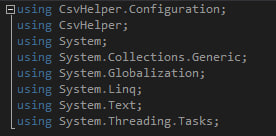
\includegraphics[width=10cm]{labs.jpg}
	\caption{\footnotesize Używane biblioteki}
	\label{fig:plotend}
\end{figure}
Na screenie widoczne są wszystkie użyte biblioteki: - CsvHelper, CsvHelper.Configuration - biblioteki dla pracy z bazą danych na CSV plikach. - Oraz w projekcie importowana biblioteka do pracy z kolekcjami(System.Collections.Generic). System zestaw podstawowch funkcji w języku C#
Zgodnie z wymaganiami projektu, realizowany jest w języku C#
\subsection{Minimalne wymagania sprzętowe}
\begin{itemize}
    \item Processor - Intel Core 2 Duo E8400
    \item Pamięć operacyjna 500 mb
    \item Potęga karty graficznej 524 mb
    \item Miejsce na dysku twardym 100 mb
\end{itemize}
% ********** Koniec rozdziału **********

\newpage
% ********** Rozdział 3 **********
\chapter{Realizowanie \&\& warstwa projektu}
\section{Diagram Gantta}
\begin{figure}[!ht]
	\centering
		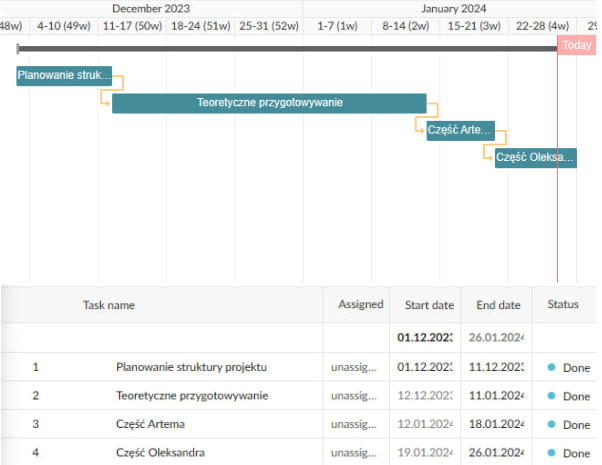
\includegraphics[width=16cm]{gantt.jpg}
  \caption{\footnotesize Realizowanie projektu}
	\label{fig:plotend}
\end{figure}
Z diagramu widać, że najpierw przez 10 dni planowaliśmy projekt i omawialiśmy, co będziemy realizowali jako pierwsza wersja aplikacji. Zaten przygotowywanie zajęło dużo czasu, po czym zaczęliśmy pisać kod projektu, najpierw Pan Artem i pozostałe realizowałem sam.
\newpage
\section{Prezentacja warstwy projektu}
\begin{figure}[!ht]
	\centering
		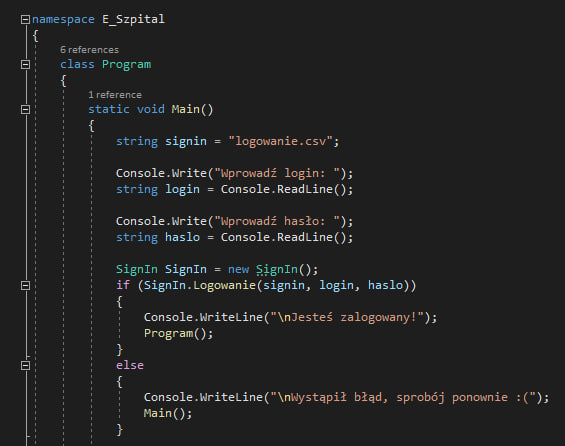
\includegraphics[width=16cm]{E-Szpital/oop1.jpg}
	\caption{\footnotesize Logowanie do aplikacji}
	\label{fig:plotend}
\end{figure}\newline
Na starcie projektu od razu wita nas logowanie, w tym celu pobieramy Login i Hasło za pomocą\\ ReadLine, a za pomocą metody Logowanie sprawdzamy czy hasło i login wpisane przez użytkownika znajdują się w bazie danych.\newpage Metoda Logowanie wygląda następująco: znajduje się w klasie SignIn, i pobiera ścieżkę do bazy loginów i haseł. Metoda tworzy tablicę z danych znajdujących się w bazie i porównuje dostępne dane z danymi wprowadzonymi przez użytkownika za pomocą foreach. Jeśli dane się zgadzają, metoda zwraca wartość true. Jeśli nie, false
\newline
\begin{figure}[!ht]
	\centering
		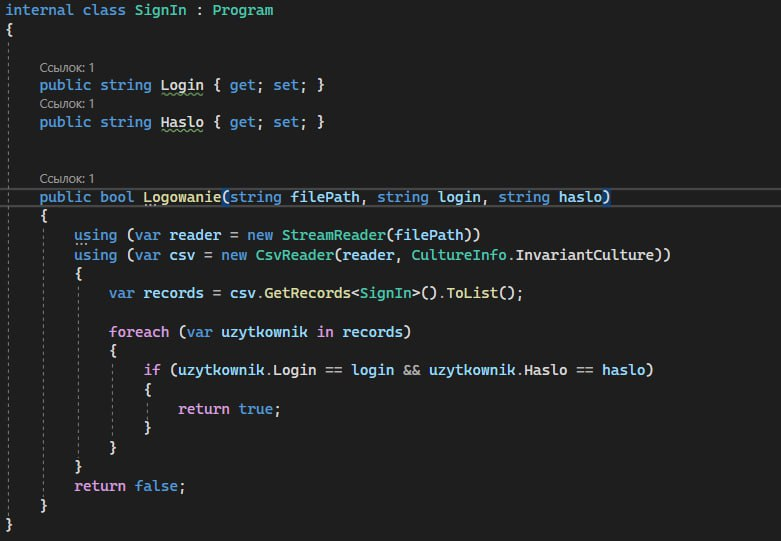
\includegraphics[width=16cm]{E-Szpital/signin.jpg}
	\caption{\footnotesize Metoda logowania}
	\label{fig:plotend}
\end{figure}\newpage
W tym miejscu znajdują się niezbędne lokalne zmienne, stworzone do wyjaśnienia aplikacji, z których plików csv pobierać lub zapisywać informacje, również lokalne zmienne do korzystania z metod, które są stworzone w klasach. \newline
\begin{figure}[!ht]
	\centering
		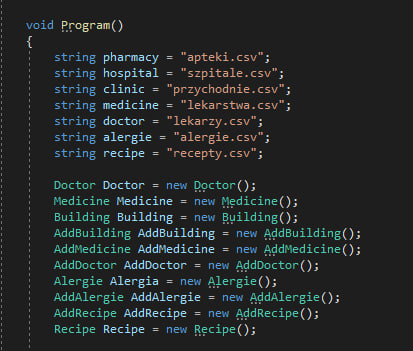
\includegraphics[width=16cm]{E-Szpital/oop2.jpg}
	\caption{\footnotesize Programowe niezbędności}
	\label{fig:plotend}
\end{figure}\newpage
Główne menu ma 8 opcje, 6 do korzystania jako użytkownik: wyświetlenie informacji o aptekach, szpitalach, przychodniach, lekach, lekarzach i alergiach. Oraz "7. Dodaj" służy do up-date`u aplikacji z możliwością dodawać nowe dane do bazy. Zwykły ReadLine do wyboru opcji z wpisanej wartości. \newline
\begin{figure}[!ht]
	\centering
		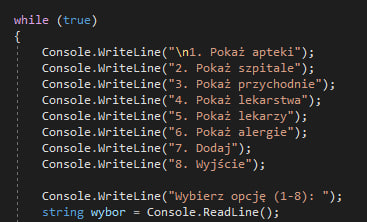
\includegraphics[width=16cm]{E-Szpital/oop3.jpg}
	\caption{\footnotesize Główne menu}
	\label{fig:plotend}
\end{figure}\newpage
Tak wygląda rozwinięcie opcji 1, czyli "Pokaż apteki", stworzone opcje wyszukiwania z nazwy, dzielnicy oraz wyświetlenie wszystkich aptek z bazy danych. W tym bloku głównie działa wszystko odwołując do metod, stworzonych w klasie "Building", które pokazane są dalej. \newline
\begin{figure}[!ht]
	\centering
		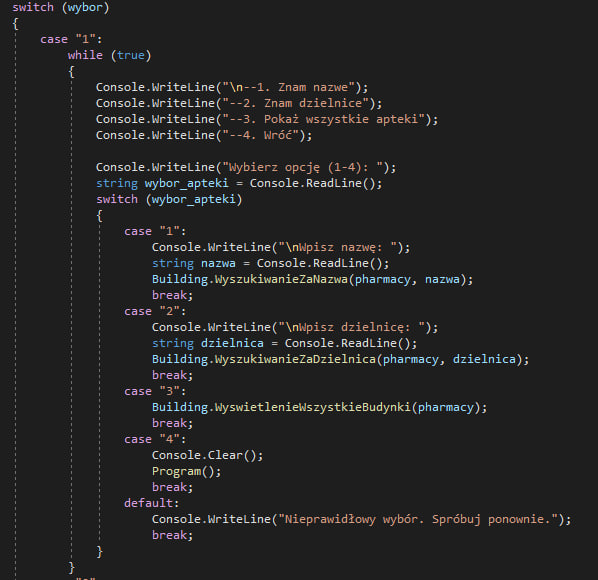
\includegraphics[width=16cm]{E-Szpital/oop4.jpg}
	\caption{\footnotesize Pokaż apteki}
	\label{fig:plotend}
\end{figure}\newpage

Biblioteki CSVhelper, CSVhelper.Configuration umożliwiają stworzenie metody do uzyskania dostępu do danych z pliku csv. Var`y reader i csv służą do wyszukiwania potrzebnego pliku, łącznie z odwołaniem do var pharmacy, pokazanego już wcześniej. Var records pobiera wpisywane dane do sprawdzania, czy są w pliku.\newline
\begin{figure}[!ht]
	\centering
		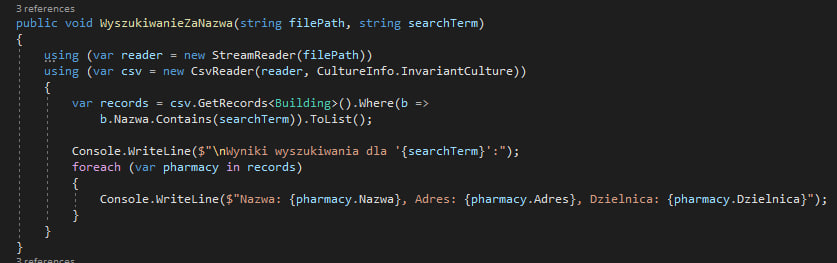
\includegraphics[width=16cm]{E-Szpital/oop5.jpg}
	\caption{\footnotesize Metoda wyszukiwania za nazwą}
	\label{fig:plotend}
\end{figure}\newline
Wyświetlenie wszystkich budynków różnie się w var records, bez sprawdzania istnienia wpisanych danych w pliku, pokazując wszystko po kolei.\newline
W podobny sposób byli napisane inne wyszukiwania z różnicami dt. danych, przykładowo leki do wyszukiwania mają atrybuty "nazwa","producent"\ i "kategoria"; lekarz - "imie", "nazwisko"\\\ i "specjalność" i t.d. Żeby zaoszędzić troche czasu pominiemy pokazywanie wykorzystanie z takich samych formuł tworzenia metod.\newline
\begin{figure}[!ht]
	\centering
		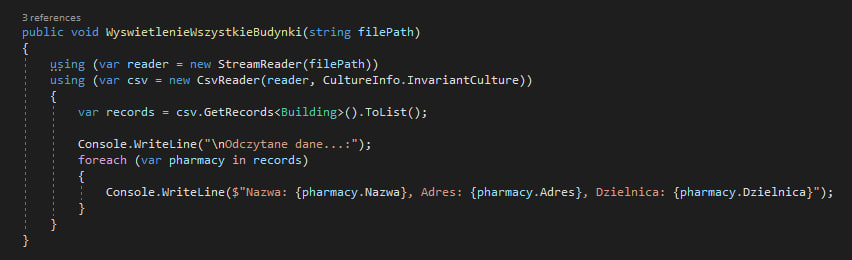
\includegraphics[width=16cm]{E-Szpital/oop6.jpg}
	\caption{\footnotesize Metoda wyświetlenia wszystkich danych}
	\label{fig:plotend}
\end{figure}\newpage
\begin{figure}[!ht]
	\centering
		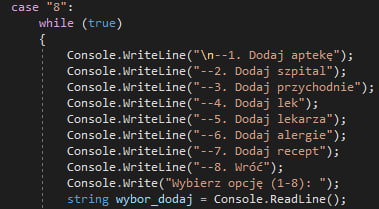
\includegraphics[width=14cm]{E-Szpital/oop7.jpg}
	\caption{\footnotesize Menu dodawania nowych danych}
	\label{fig:plotend}
\end{figure}\newline
Tak samo za pomocy bibliotek CSVhelper, CSVhelper.Configuration stworzone są metody do dodania nowej informacji do plików, z których korzysta aplikacja, do których tutaj wpisane są odwołania.\newline
\begin{figure}[!ht]
	\centering
		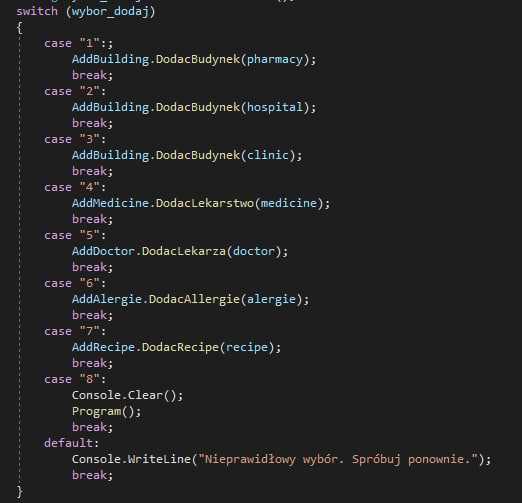
\includegraphics[width=14cm]{E-Szpital/oop8.jpg}
	\caption{\footnotesize Odwołania do metod}
	\label{fig:plotend}
\end{figure}\newpage
\begin{figure}[!ht]
	\centering
		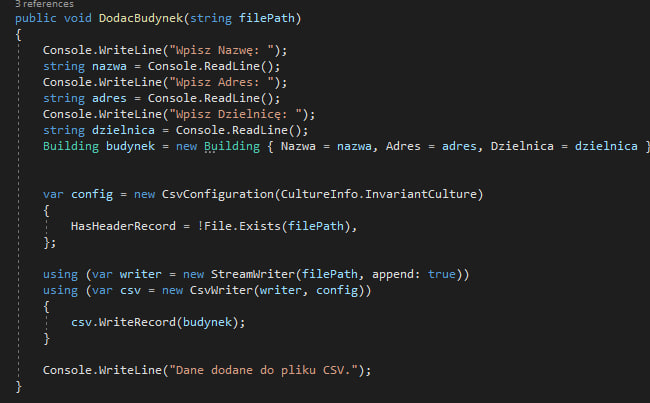
\includegraphics[width=14cm]{E-Szpital/oop9.jpg}
	\caption{\footnotesize Metoda dodawania nowych danych}
	\label{fig:plotend}
\end{figure}\newline
Podobnie do tego screenu, używając readline do pobierania wpisywanych danych od użytkowniku, stwarza się obiekt klasy "Building" i za pomocy csvhelper rzucamy ten obiekt do bazy danych.\newpage

\subsubsection{Żródła plików}
\begin{figure}[!ht]
	\centering
		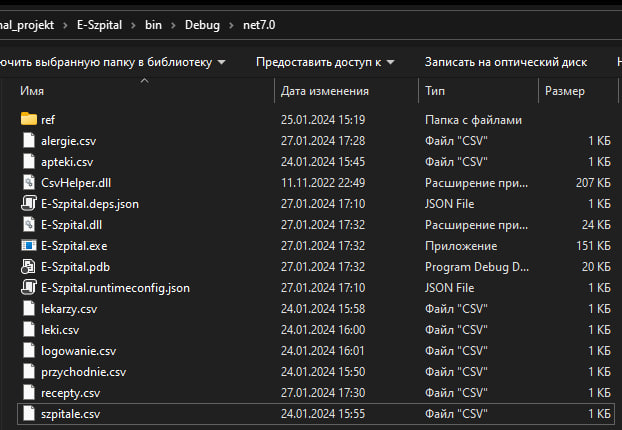
\includegraphics[width=16cm]{E-Szpital/net7.jpg}
	\caption{\footnotesize Pliki używane aplikacją}
	\label{fig:plotend}
\end{figure}\newline
\begin{figure}[!ht]
	\centering
		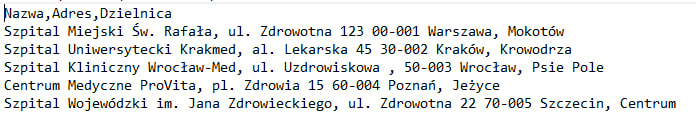
\includegraphics[width=16cm]{E-Szpital/szpital.jpg}
	\caption{\footnotesize Tekst w pliku szpital.csv}
	\label{fig:plotend}
\end{figure}\newline
I tutaj widoczne jest, jak wygląda tekst, który rozumie aplikacja i biblioteki powiązanie z csv. W podobny sposób zrobione są pozostałe.
\newpage\subsection{Podalsze plany}
Dalsze rozwinięcie projektu łączy w sobie pracę nad interfejsem, funkcjonalnością, dodawanie nowych metod i potencjalnie testowanie gotowej wercji (do tego jeszcze długo).
% ********** Koniec rozdziału **********

\newpage

% *************** Bibliografia ***************
\begin{thebibliography}{6}
\addcontentsline{toc}{chapter}{Bibliografia}
%dodanie wpisu do spisu bibliograficznego

\bibitem{www-1} https://ec.europa.eu/eurostat/statistics-explained/ z dnia 26.01.2024

\bibitem{etykieta1}Internetowe strone, wielkie i najlepsze

\end{thebibliography}
\newpage

% *************** Zakończenie ***************
% *************** Zakończenie ***************

%spis rysunków
\addcontentsline{toc}{chapter}{Spis rysunków}
\listoffigures
\newpage

%streszczenie
\addcontentsline{toc}{chapter}{Streszczenie}
\noindent
{\footnotesize{}\textbf{Wyższa Szkoła Informatyki i Zarządzania z siedzibą w Rzeszowie\\
Kolegium Informatyki Stosowanej}
\vspace{30pt}

\begin{center}
\textbf{Projekt z przedmiotu Programowanie Obiektowe}\\
\temat
\end{center}

\vspace{30pt}
\noindent
\textbf{Autor: \autor
\\Promotor: \promotor
}
\vspace{120pt}

\noindent
\textbf{The University of Information Technology and Management in Rzeszow\\
Faculty of Applied Information Technology}
\vspace{30pt}

\begin{center}
E-Szpital
\end{center}

\vspace{30pt}
\noindent
\textbf{Author: \autor
\\Supervisor: \promotor
}
\vspace{40pt}
\\This project was made out of pure will to help people, help someone else, and help in general.
}

% *************** Koniec pliku back.tex ***************


\end{document}
% *************** Koniec pliku szablon.tex ***************
